\documentclass[11pt]{article}
\usepackage[margin=1in]{geometry}                % See geometry.pdf to learn the layout options. There are lots.
\geometry{letterpaper}                   % ... or a4paper or a5paper or ... 
%\geometry{landscape}                % Activate for for rotated page geometry
%\usepackage[parfill]{parskip}    % Activate to begin paragraphs with an empty line rather than an indent
\usepackage[breaklinks=true, colorlinks=true, linkcolor=red, urlcolor=blue, citecolor=black]{hyperref}
\urlstyle{rm}
\usepackage{mathptmx}
\usepackage{graphicx}
\usepackage{amssymb}
\usepackage{epstopdf}
\usepackage{color}
\usepackage{sidecap}
\usepackage{authblk}
\usepackage{booktabs}
\usepackage[font=small,labelfont=bf]{caption}
\usepackage{enumitem}
\usepackage{wrapfig}
\DeclareGraphicsRule{.tif}{png}{.png}{`convert #1 `dirname #1`/`basename #1 .tif`.png}
\pagestyle{plain}

\def\bfr{\bf\color{red}}
\def\geohub{{\tt geohub}}
\def\resp{respectively}
\def\selah{SELAH}

\begin{document}
%\maketitle

\begin{center}
	\Large\bf Unsheltered Homelessness in Hollywood Is Down from January 2020 Levels\\
	\vspace{1ex}
	{\normalsize\rm Louis Abramson, PhD, and Brian Kohan 
	for the \href{http://www.hollywood4wrd.live}{\it Hollywood4WRD Coalition} \\ \today -- {\bfr NOT FOR PUBLIC DISTRIBUTION}}

%	\vspace{1em}

%	{\large\it Summary}	
\end{center}

\noindent {\bf Summary:} The number of people experiencing unsheltered homelessness in both Hollywood 
and East Hollywood has fallen since the last LAHSA Point-In-Time (PIT) count in January 2020. %(1/23)
Using a complete census of these communities from 25 February 2021, we estimate decreases of 
$11\%\pm9\%$ and $15\%\pm12\%$ (90\% CI), \resp, suggesting at least a 93\% chance of a decline.
%assuming no changes in average dwelling occupancies, 

A $\sim$30\% reduction in persons seen on the street drives this change (Figure \ref{fig:rawCounts})---enough 
to lower {\it raw counts} of individuals and dwellings in about a third of census tracts (Figure \ref{fig:tcomp}). 
This trend is independent of whether counters were professionals or volunteers and is larger than what data acquisition 
errors will admit. A qualitative decline in unsheltered living is thus likely to persist even given reasonable 
changes in demographic weights, which at least one preliminary survey suggests may be modest. 
%Only seven tracts saw significant increases in raw counts, with makeshift dwellings the only category to increase in both CoCs. 
%All data are available to support future analyses incorporating such information.

Data from the Coordinated Entry System will reveal whether homelessness has declined in toto, or if
COVID-related initiatives reduced only the portion of people living unsheltered in Greater Hollywood.

\begin{figure*}[h]
	\centering
	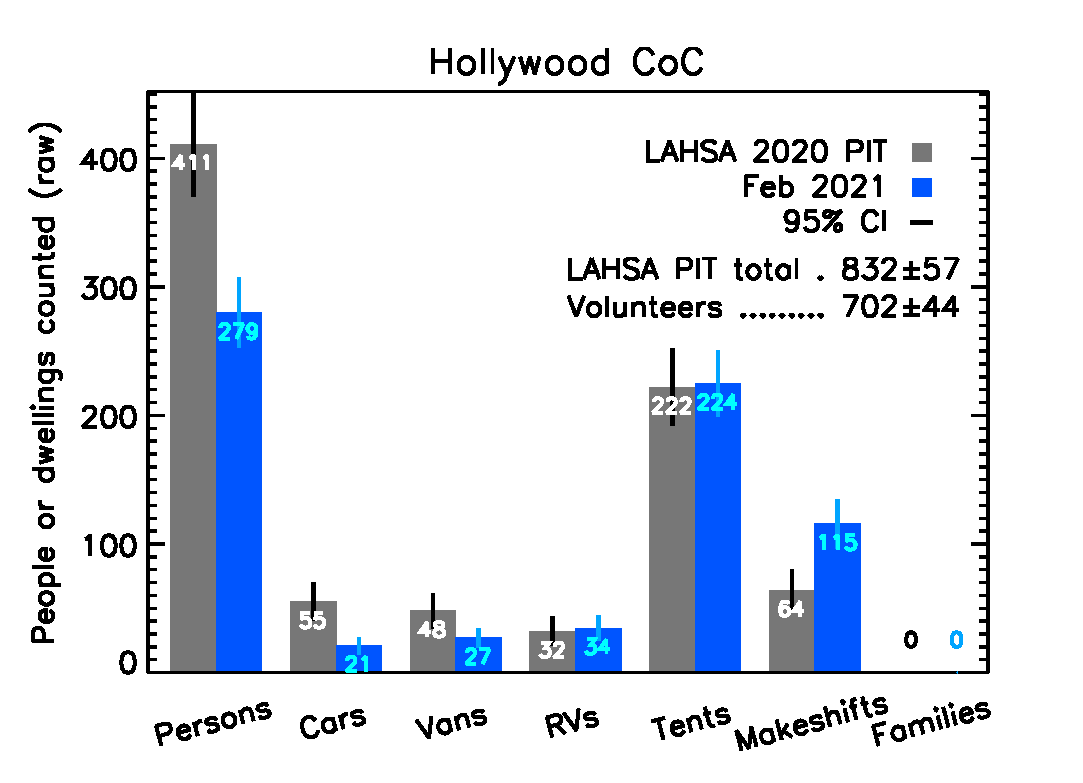
\includegraphics[width = 0.47\textwidth, trim = 1cm 0cm 0cm 0cm]{Hwood2021Bars}
	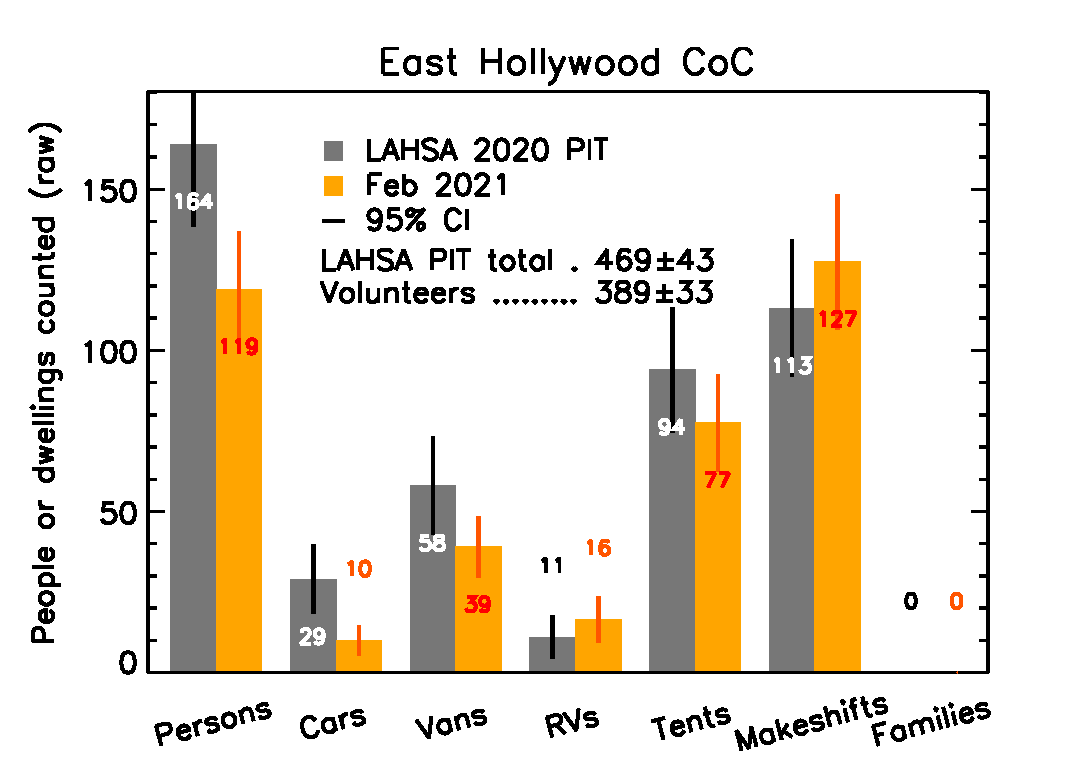
\includegraphics[width = 0.47\textwidth, trim = 1cm 0cm 0cm 0cm]{Eho2021Bars}
	\caption{Raw tallies of unsheltered persons and dwellings in Hollywood (left) and E.~Hollywood
			(right) from the 2020 (grey) and 2021 (colors) Point-In-Time counts. Persons, cars, 
			and vans declined in both communities, RVs and tents remained flat, with makeshift 
			structures the lone category to show a potential common increase. 
			These areas were surveyed almost entirely by independent teams.}
	\label{fig:rawCounts}
\end{figure*}

\begin{table*}[h!]
\caption{Greater Hollywood Unsheltered Data and Population Estimates}
\resizebox{\linewidth}{!}{%
\begin{tabular}{lcccccccccc}
\toprule
 & Adult & TAY & Car & Van & RV & Tent & Makeshift & {\bf 2021 Total} & {\bf 2020 Total} & {\bf Difference} \\ \cmidrule{1-11}
{\bf Hollywood} \\ %\cmidrule{1-1}
Counts & 277 & 2 & 21 & 27 & 34 & 224 & 115 & {\bf 702} & {\bf 831} & $\bf -15\%$ \\
Inhabitants & 277 (27) & 2 (5) & 32 (11) & 49 (13) & 50 (14) & 332 (29) & 195 (24) & {\bf 937 (93)} & {\bf 1058} & $\bf -11\%\,(9\%)$\\% (76)
Category share & 30\% (3\%) & 0\% (0\%) & 3\% (1\%) & 5\% (1\%) & 5\% (1\%) & 35\% (3\%) & 21\% (3\%) & -- & -- & -- \\ \cmidrule{1-11}
{\bf East Hollywood} \\ %\cmidrule{1-1}
Counts & 114 & 4 & 10 & 39 & 16 & 77 & 127 & {\bf 389} & {\bf 469} & $\bf -17\%$ \\
Inhabitants & 114 (19) & 4 (4) & 15 (8) & 70 (15) & 24 (9) & 115 (19) & 216 (23) & {\bf 557 (83)} & {\bf 656} & $\bf -15\%\,(12\%)$\\% (60)
Category share & 20\% (3\%) & 1\% (1\%) & 3\% (1\%) & 13\% (3\%) & 4\% (2\%) & 20\% (3\%) & 39\% (4\%) & -- & -- &--
\\ \bottomrule
\end{tabular}
}
\caption*{Parentheses denote 95\% uncertainties (binomial in the case of the categories). Uncertainties larger than estimates 
imply that only upper limits are available. No unaccompanied minors or families were observed; ``Persons'' are TAY+Adults.}
\label{tbl:summary}
\end{table*}

\noindent {\bf Context:} Government, nonprofit, and volunteer organizations in Hollywood\footnote{Including
{\it \href{https://chnc.org}
{The Central Hollywood Neighborhood Council}, \href{https://thecenterinhollywood.org}{The Center
at Blessed Sacrament}, \href{https://www.myfriendsplace.org/}{My Friend's Place}, Hang Out Do Good, \href{https://hollywood4wrd.live}
{Hollywood4WRD}, \href{https://www.covenanthouse.org/spring-meal-match?sourceid=2483460&origin=DHQEI2109EZI0N&utm_source=2103marchmealmatchweb&utm_medium=cpc&utm_campaign=FY21MarchMealMatch&utm_content=bsd2103marchmealmatchweb&gclid=CjwKCAiAp4KCBhB6EiwAxRxbpJA2yM7lM2tyAqjVALZgBGvjnhobCJJ0XmuELFDXzM5xxZ0BqyX1ChoCLi0QAvD_BwE}{Covenant House}}, and various resident organizers.} conducted 
a PIT enumeration of people experiencing unsheltered homelessness to compensate for 
the \href{https://laist.com/latest/post/20201209/LAHSA-cancels-2021-homeless-count-los-angeles-covid-19}
{cancellation} of the official 2021 countywide count. All 39 US Census tracts in the LAHSA-recognized Hollywood 
and East Hollywood communities were surveyed on 25 February (Figure \ref{fig:tcomp}). Nine tracts---comprising 
$\sim$43\% of total individuals and dwellings identified---were counted by professional outreach teams during the 
day. The remainder were surveyed by car-based volunteer teams beginning at 7:00 PM.

Each volunteer team was assigned two tracts in either Hollywood or E.~Hollywood. Since 32 teams 
turned-out, each tract was counted by at least two independent teams. Such redundancy increased the 
count's accuracy and enabled better error assessments. Tracts surveyed by professionals were 
counted only once. Zero volunteer teams and only professional team counted tracts in both 
communities, enabling trends to be cross-validated across nearly independent datasets.

Year-on-year trends are consistent across communities and between volunteer- and professionally counted tracts.
Six tracts saw significant inferred population increases; 14 saw significant declines. The largest 
increase was observed by volunteers; the largest decrease by professionals (both in E.~Hollywood).\\

\begin{figure*}[h]
	\centering
%	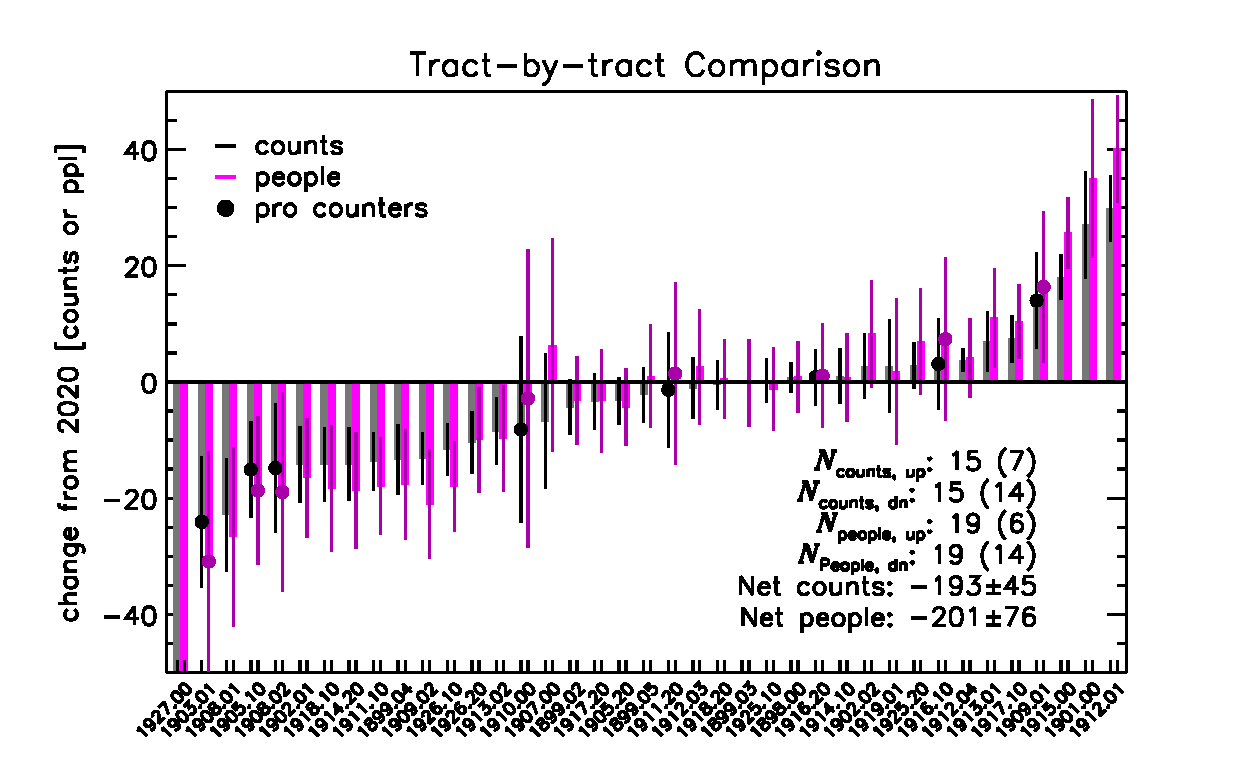
\includegraphics[width = 0.8\textwidth, trim = 0cm 0cm 0cm 0cm]{tractsYrYr}
	\includegraphics[width = 0.8\textwidth, trim = 0cm 0cm 0cm 0cm]{map}
	\caption{Map of the volunteer PIT survey area with census tracts colored by inferred 
			changes in total unsheltered population from 2020 ({\bfr colors}).
			Hollywood (21 tracts) stretches from Crescent Heights/Franklin to 
			Western /Melrose; E.~Hollywood (18 tracts) from Western/Hollywood 
			Blvd to Hoover/Beverly Blvd. The largest changes were in E.~Hollywood,
			with tract 1912.01 (NE, volunteer-tallied) rising by 40 people and 1927.00 
			(SE, pro-tallied) falling by over 120 people. Subsequent cross-checks of both
			tracts support the accuracy of their PIT counts. {\bfr This is a placeholder figure}.}
	\label{fig:tcomp}
\end{figure*}

\begin{figure*}[h]
	\centering
	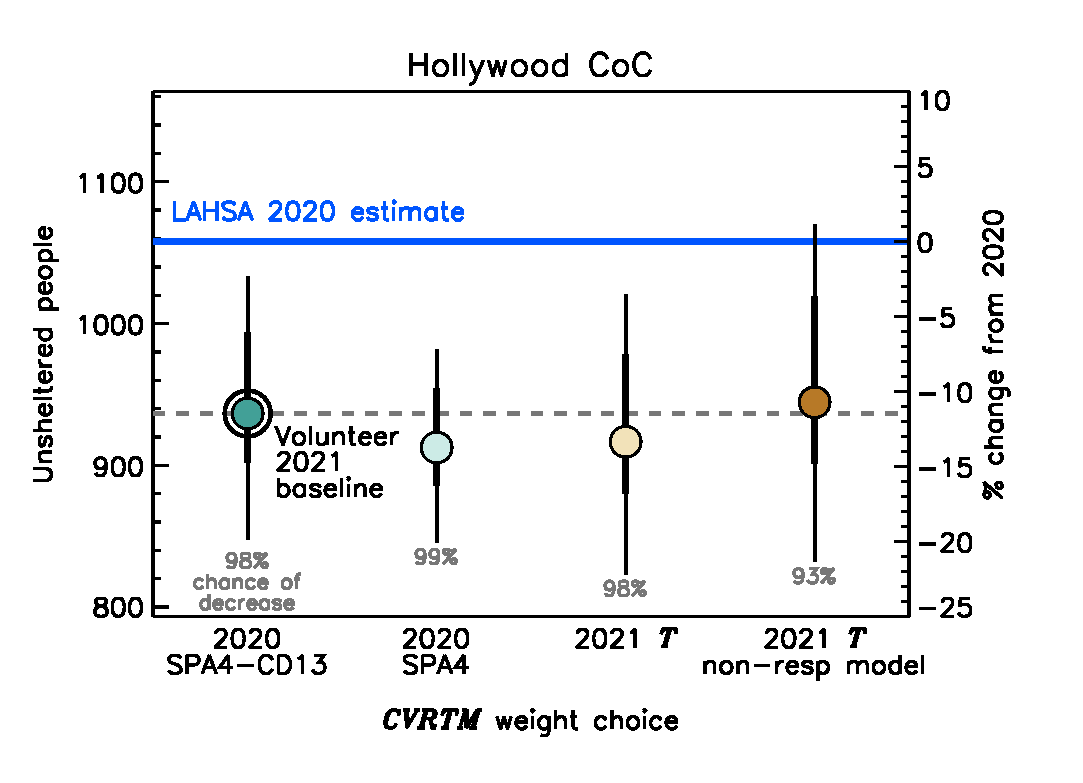
\includegraphics[width = 0.48\textwidth, trim = 1cm 0cm 0cm 1cm]{hwoodFinal}
	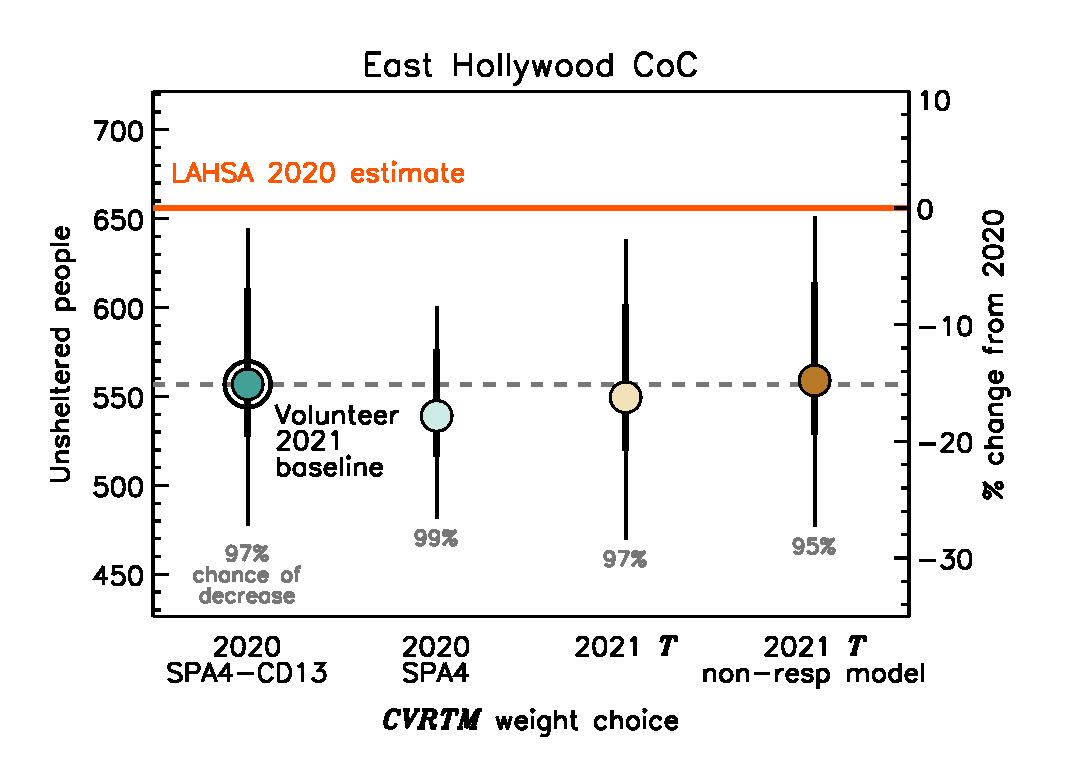
\includegraphics[width = 0.48\textwidth, trim = 1cm 0cm 0cm 1cm]{ehoFinal}
	\caption{}
	\label{fig:wtComp}
\end{figure*}

\noindent {\bf Results and uncertainties:} The population inferences in Table \ref{tbl:summary} and 
Figure \ref{fig:wtComp} reflect 10,000 Monte Carlo resamplings of the survey data with 
counts perturbed randomly by their uncertainties. Counts for cars, vans, RVs, tents, and 
makeshift dwellings (CVRTM) were additionally boosted by the relevant demographic weights 
perturbed by their own uncertainties. The baseline case---quoted in Table \ref{tbl:summary} and 
shown in teal in Figure \ref{fig:wtComp}---adopts the 2020 
\href{https://www.lahsa.org/documents?id=4635-usc-2018-2020-multipliers-and-estimates-overview}
{SPA4/CD13 CVRTM weights} underpinning the latest official Hollywood and E.~Hollywood 
\href{https://www.lahsa.org/documents?id=4686-2020-greater-los-angeles-city-community-homelessness-report-service-planning-area-4.pdf}
{Community Summaries}, from which we also draw raw 2020 person and CVRTM tallies. Those inferences yield 
$936\pm92$ and $556\pm83$ people experiencing unsheltered homelessness, \resp\ (90\% CI). Modifying the weights
to their 2020 \href{https://www.lahsa.org/documents?id=4693-2020-greater-los-angeles-homeless-count-cvrtm-conversion-factors}
{SPA4-wide} values or using data from in-person surveys of tent-dwellers in Hollywood has no
significant effect (Figure \ref{fig:wtComp}).

Nevertheless, the CVRTM weights represent systematic uncertainties: underestimating them would bias
our population estimates low and perhaps erode the declines we infer in both communities. We encourage robust
efforts to ascertain current CVRTM occupancies, but the declines in unweighted counts are large enough that 
the changes from 2020 must be substantial to bring our estimate in-line with last year's. All else being equal, 
the average tent would need to shelter (2.8) 2 people in (East) Hollywood vs.\ 1.5 people in 2020. Meanwhile, 
the average makeshift structure would need to shelter (2.5) 2.7 people vs.\ 1.7 people in 2020. Notwithstanding
a 28 February survey of tents in Hollywood that yielded a tent occupancy consistent with the 2020 value, 
such 30\%--90\% increases {\it in the mean} seem unlikely, especially when known tent distribution efforts 
during COVID would push in the opposite direction.\footnote{Given the high proportion of people dwelling in tents
and makeshift structures, the $T$ and $M$ weights are the largest potential error sources in this analysis. While 
surveys of the full 2021 PIT area have not been conducted, \href{https://selahnch.org}{\selah} outreach teams 
surveyed of 47 tents (38 responses) in Hollywood on 28 February, yielding a mean occupancy of 
$T=1.39\pm0.14$ people per tent, or $T=1.50\pm0.22$ when non-responses are modeled. While $M$ was
not estimated, both $T$ values are consistent with the official 2020 weight of $T=1.48\pm0.11$.}

Numerous cross-checks give us confidence that the raw counts are accurate:
\begin{enumerate}
%	\setlength{\itemsep}{-1ex}
	\item Comparisons of the PIT count's 37 duplicate tract measurements suggest per-tract and per-category
		counting uncertainties are consistent with the random errors built into the analysis.
%		\begin{itemize}
%			\item Tract 1901.00---the only outlier in the above comparisons---was independently recounted 
%				14 hours after the PIT count with results consistent with the average of the volunteer teams' 
%				results.
%			\item Tract 1912.01---largest increase---was independently recounted on 27 Feb.\ circa 
%				12:00 PM with results similarly consistent with the PIT teams' assessments.
%			\item Tract 1927.00---largest decrease---was independently recounted on 4 March at 
%				8:30 AM with results lower than the PIT's assessment. This especially dense tract was originally 
%				surveyed on foot by outreach professionals, however, with the recount was performed by a car-based
%				volunteer. The cross-check therefore suggests only that the PIT data are not biased in ways that
%				would induce an artificial year-on-dear decline.				
%		\end{itemize}
	\item External data from \href{https://hollywoodpartnership.com/}{\it The Hollywood Partnership} 
		from 19 Feb.\ are consistent with both the PIT count in a common tract (1902.02) and an independent 
		recount of that entire geography performed 28 Feb. They also show a decline from past values.
	\item Comparisons of tracts counted by volunteer and professional teams show consistent trends.
	\item Comparisons of counts in Hollywood and E.~Hollywood show consistent trends.% (reduced individuals, flat
%		or marginally higher dwelling counts).
	\item Four tracts monitored by \selah\ since May 2020 show similar declines. One of these is E.~Hollywood's tract 
		1912.01---home to the largest gain---whose \selah\ estimate agrees with our PIT value.% in unsheltered homelessness.
\end{enumerate}

%		   P	C     V	    R	 T     M
%1901.00 -- 50    8    5.5   1     6      4 -- 2021, raw
%1901.00 -- 36    4     6     0     8      2 -- 26 Feb ABRAMSON 9.00 AM
%
%1927.00 -- 48    1      5     0    53    70 -- 2020, raw
%1927.00 -- 20    0     0     7     6     54 -- 2021, raw
%1927.00 -- 15     0     9     5    14    21 -- 4 Mar 2021 ABRAMSON 8.45 AM
%
%1912.01 --  18.5  0.5  3.5  1.5  5.5  12 -- 2021, raw
%1912.01 --  21     0      4     1     8      6  -- 27 Feb ABRAMSON 12.15 PM
%
%1902.02 -- 9      --     --     --     8   5.5 -- 2021, raw
%1902.02 -- 9      --     --     --    17    --  -- BID 2/19

%The pro/vol trends are consistent everywhere except tract 1927.00, 
%			where pro counts dropped significantly more for both individuals and dwellings (esp.\ 
%			tents). 1927.00 comprises 22\% of total counts in E.~Hollywood. Unsheltered 
%			homelessness in that CoC was flat or rose slightly outside of that tract.}
%{\bfr 1927.00 is the tract with the PATH Madison PSH. Phase II opened in Jan 2020---leasing began May 
%2020---and is 120 units, some of which were filled from nearby folks but I dunno how many. LEA recounted 
%this tract 4 March at $\sim$9:00 AM and found 94 total population vs.\ pro's 129. Only place where
%LEA counted more objects was vans. Adding that to the pro total adds 16 people (9 vans).

All of the above suggests that our results are reliable both quantitatively and qualitatively.\\

\noindent {\bf Comments:} The decline we find vs.\ 2020 is largely driven by a $\sim$30\% 
drop in observed unsheltered individuals in both Hollywood and E.~Hollywood. This reduction
may partially be attributable to government initiatives aimed at moving people indoors (Project Roomkey, 
various emergency shelters) and staunching inflow into homelessness (eviction moratoria). Examining 
Project Roomkey, \href{https://www.lahsa.org/documents?id=4672-2020-homeless-count-council-district-13}
{CD13's} share of \href{https://www.lahsa.org/documents?id=4585-2020-greater-los-angeles-homeless-count-los-angeles-continuum-of-care-coc-}{LA County's total senior unsheltered population} (6.5\%) implies that perhaps 100 of Project Roomkey's 
\href{https://projectroomkeytracker.com/}{1608 occupied rooms} were filled with Greater Hollywood 
residents on the night of the PIT count---enough to account for about half the decline we infer. 
The opening of at least one {\it A Bridge Home} in Los Feliz---whose catchment area includes Hollywood---may 
also have contributed, as may the opening of 120 permanent supportive housing units by PATH in May 2020 
in tract 1927.00. While all of the latter did not go to local unhoused residents, some may have, and may 
therefore have helped drive that tract's large observed decline. 

Data from the Coordinated Entry System 
should constrain the above possibilities, and so reveal whether homelessness writ-large has fallen since 2020 or 
simply the unsheltered share in Hollywood.

If the numbers have fallen, however, COVID-related closures of restaurants and other facilities that
once provided basic necessities (food, hygiene) to unhoused people have substantially degraded conditions 
for those left on the street. Reduced sanitation activities and access to mental health and drug treatment centers 
{\bfr (VERIFY)} have only exacerbated those challenges. Hence, while these data may support the efficacy of 
programs designed to reduce street homelessness, they do not suggest that the qualitative state of homelessness 
in Hollywood has improved. In the fight to rebuild lives---as well as build homes---such a fact must not be forgotten.

%HOLLYWOOD -- Zero delta requires CVRTM mean occupancies of:\\
% - 5.00 ppl/car (from 1.51)\\
% - 5.00 ppl/van (from 1.77)\\
% - 4.95 ppl/RV (from 1.42)\\
% - 2.03 ppl/tent (from 1.48)\\
% - 2.73 ppl/mkshft (from 1.68)\\
%
%EAST HOLLYWOOD -- Zero delta requires CVRTM mean occupancies of:\\
% - 5.00 ppl/car (from 1.51)\\
% - 4.33 ppl/van (from 1.77)\\
% - 5.00 ppl/RV (from 1.42)\\
% - 2.78 ppl/tent (from 1.48)\\
% - 2.45 ppl/mkshft (from 1.68)


% ------ SUMMARY for HWOOD ------ 
%
%Total People (90%CI) .   936+/-92
%Fraction vs. last yr .   0.89+/-0.09
%Total counts..........   702
% > Adults    : 277 (39%), 277, (29%)
% > TAY       :   2 ( 0%),   2, ( 0%)
% > Minors    :   0 ( 0%),   0, ( 0%)
% > Cars      :  21 ( 2%),  31, ( 3%)
% > Vans      :  27 ( 3%),  47, ( 5%)
% > RVs       :  34 ( 4%),  49, ( 5%)
% > Tents     : 224 (31%), 330, (35%)
% > Makeshifts: 115 (16%), 193, (20%)
% > Families  :   0 ( 0%),   0, ( 0%)
%% Compiled module: MINMAX.
%Min/max ppl/tract ..... 0, 169
%Min/max counts/tract .. 0, 123
%
% ------ SUMMARY for EHO ------ 
%
%Total People (90%CI) .   556+/-83
%Fraction vs. last yr .   0.85+/-0.13
%Total counts..........   389
% > Adults    : 114 (29%), 114, (20%)
% > TAY       :   4 ( 1%),   4, ( 0%)
% > Minors    :   0 ( 0%),   0, ( 0%)
% > Cars      :  10 ( 2%),  14, ( 2%)
% > Vans      :  39 (10%),  68, (12%)
% > RVs       :  16 ( 4%),  23, ( 4%)
% > Tents     :  77 (19%), 114, (20%)
% > Makeshifts: 127 (32%), 214, (38%)
% > Families  :   0 ( 0%),   0, ( 0%)
%Min/max ppl/tract ..... 6, 129
%Min/max counts/tract .. 5, 87


%\begin{wrapfigure}{r}{0.5\linewidth}
%	\centering
%	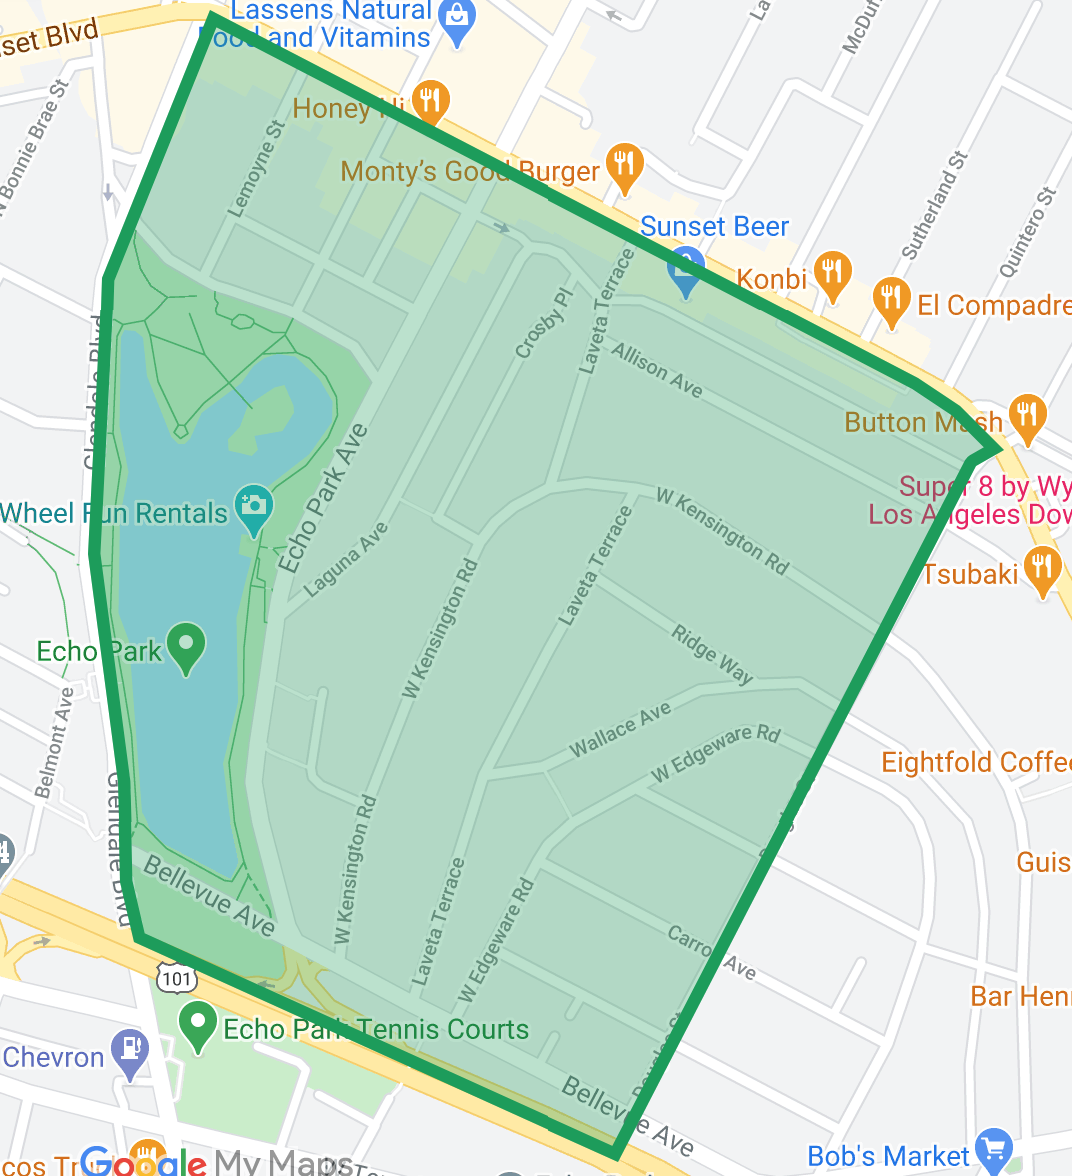
\includegraphics[width=\linewidth]{t1975}
%	\caption{US Census tract 1975.00.}
%	\label{fig:tract}
%\end{wrapfigure}
%\noindent {\bf Context:} \selah\ volunteers performed two recounts of US Census tract 1975.00 
%on 2 August and 18 October 2020 (Figure \ref{fig:tract}). This tract contains Echo Park Lake and various 
%CalTrans lands. The results of both surveys were statistically identical except for the estimate of vans, 
%which rose from $14\pm3$ to $25\pm5$ between counts. Our final individual/dwelling statistics 
%(Table \ref{tbl:rawData}) and total population estimates (Figure \ref{fig:results}) reflect the average 
%of those assessments.\\

%{\bfr KANAGI: ``we've seen a visual drop; dunno where they went but...'' On 2/18 they found 136 
%total tents in the BID vs our 127 (I haven't vetted the rest of the lines; that's just 12\# hot so w/e). (Also 99
%ppl compared to our 89, and 7 vehicles to our 10 and we weren't tracking those as hard as tents.) 
%On the 5th, they counted 163. That's a 17\% decline in 2 weeks, a little more that what we've seen year on year.
%Suggests maybe something happened in early Feb.? -- 3/2 @ 9:55 AM. The tent+mkshft count in 1902.02 is also 
%right on..}

%Only seven tracts saw significant increases in raw counts, with makeshift dwellings the only category to increase in both CoCs. 

%
%
%Cars and vans are hard to count, but there's no evidence of a bias. I repeated the most deviant tract the next day, 
%and another tract the day after that. In the latter case, both of my estimates were 0.5 units off the mean, in the 
%former, vans were at that level and I counted fewer cars. Brian and I also recovered a consistent amount of vehicles 
%with the BID (10 vs. their 6 separated by 20+ days). The rest of the tracts show a mean inter-counter bias of 0.6 
%cars (0.4 std.~err) and 1.24 ($0.76\sigma$) vans across all tracts, which should be accounted for in the MC.


% Pro teams counted areas comprising $\sim$43\% of the total raw counts. Three out of these 4 tracts 
% were counted by Covenant House teams, but 1927.00 has the largest drop of any tract and is Elyse 
% from The Center. That tract is basically responsible for the entire decline in E.~Hollywood, and most 
% of that is in reduced tents, so we should 	talk to these teams.


\end{document}  